% To rebuild the .pdf from this source, use something like the following
%	latex quickref.tex
%	dvips -t letter -f < quickref.dvi >| quickref.ps
%	ps2pdf -sPAPERSIZE=letter quickref.ps
\documentclass[12pt]{article}
\usepackage[utf8]{inputenc}
\usepackage{lscape}
\usepackage{setspace}
\usepackage{graphicx}
\usepackage{multicol}
\usepackage[normalem]{ulem}
\usepackage[spanish]{babel}
\usepackage{color}
\usepackage{hyperref}

\textheight=9in
\textwidth=7.5in
\headheight=0pt
\headsep=0pt
\topmargin=0in
\oddsidemargin=-0.4in
\evensidemargin=-0.6in
\parindent=0pt
\parsep=1pt
\pagestyle{empty}

\date {}

\makeatother

\begin{document}
	\begin{landscape}

%	\textit{Dan Kuester's all-leather}

	\begin{center}
	\begin{minipage}[m]
		{1in}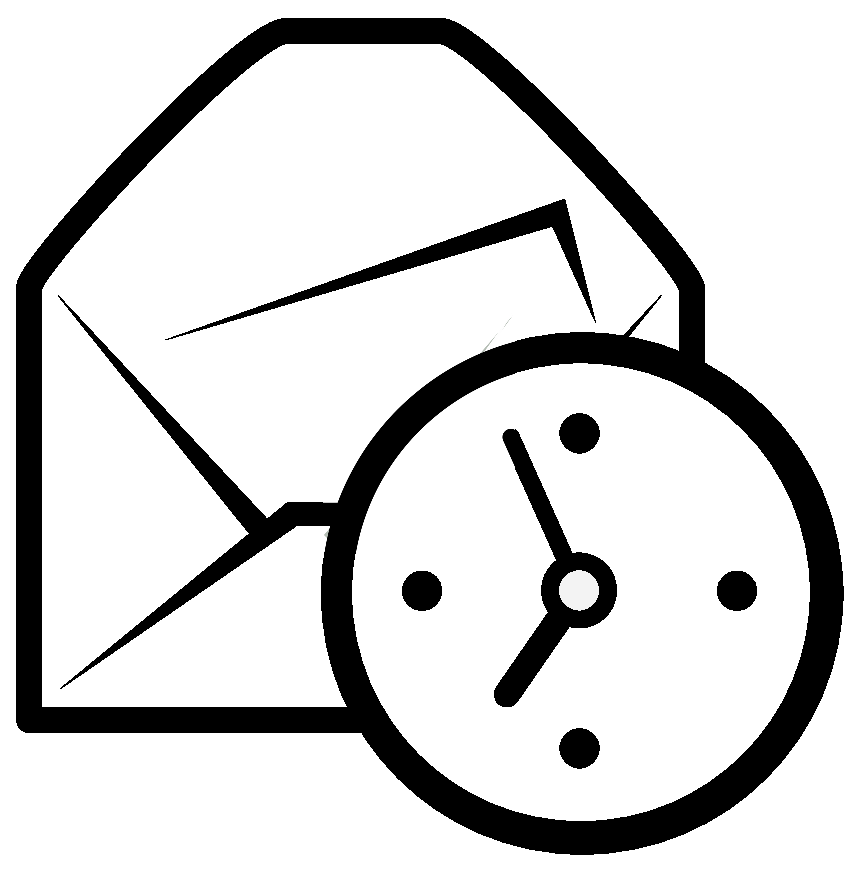
\includegraphics[height=0.9in]{../evolution-logo.eps}\hspace{5mm}
	\end{minipage}
	\hspace{5mm}
	\textbf{\Huge{Tarjeta de referencia rápida de Evolution}}
	\end{center}

	\begin{center}
	\begin{multicols}{2}
	\section*{Global}
	\begin{tabular*}{4in}{rp{1.5in}}
		\textit{\textbf{Componentes}}		&					\\
		Correo					& \textbf{Ctrl+1}			\\
		Contactos				& \textbf{Ctrl+2}			\\
		Calendario				& \textbf{Ctrl+3}			\\
		Tareas					& \textbf{Ctrl+4}			\\
		\vspace{1.5mm}
		Notas					& \textbf{Ctrl+5}			\\
		\textit{\textbf{Controles}}		&					\\
		Elemento nuevo en el modo actual	& \textbf{Ctrl+N}			\\
		Cambiar el foco entre los paneles	& \textbf{F6}				\\
		Limpiar la barra de búsqueda		& \textbf{Mayús.+Ctrl+Q}		\\
		Cerrar ventana				& \textbf{Ctrl+W}			\\
		Abrir ventana nueva			& \textbf{Mayús.+Ctrl+W}		\\
		\vspace{1.5mm}
		Salir de Evolution			& \textbf{Ctrl+Q}			\\
		\textit{\textbf{Selección}}		&					\\
		Imprimir selección			& \textbf{Ctrl+P}			\\
		Guardar selección			& \textbf{Ctrl+S}			\\
		Borrar selección			& \textbf{Supr} o \textbf{Retroceso}	\\
		Mover correo/contactos a carpeta	& \textbf{Mayús.+Ctrl+V}		\\
		Copiar correo/contactos a carpeta	& \textbf{Mayús.+Ctrl+Y}		\\
	\end{tabular*}
	\section*{Componentes de contactos/notas}
	\begin{tabular*}{4in}{rp{1.5in}}
		\textit{\textbf{Comandos generales}}	&					\\
		Contacto nuevo				& \textbf{Mayús.+Ctrl+C}		\\
		Lista de contactos nueva		& \textbf{Mayús.+Ctrl+L}		\\
		Nota nueva				& \textbf{Mayús.+Ctrl+O}		\\
	\end{tabular*}
%	{\\ \vspace{5mm} \footnotesize \textit{* denotes the feature may not be implemented yet}}
	\section*{Componente de correo}
	\begin{tabular*}{4in}{rp{1.5in}}
		\textit{\textbf{Comandos generales}}	&					\\
		Mensaje nuevo				& \textbf{Mayús.+Ctrl+M}		\\
		\vspace{1.5mm}
		Enviar/Recibir mensajes			& \textbf{F12}				\\
		\textit{\textbf{Selección}}		&					\\
		Aplicar filtros				& \textbf{Ctrl+Y}			\\
		Abrir en una ventana nueva		& \textbf{Retorno} o \textbf{Ctrl+O}	\\
		\vspace{1.5mm}
		Reenviar selección			& \textbf{Ctrl+F}			\\
		\textit{\textbf{Panel de lista de mensajes}} &					\\
		Siguiente mensaje no leído		& \textbf{.} o \textbf{]}		\\
		\vspace{1.5mm}
		Anterior mensaje no leído		& \textbf{,} o \textbf{[}		\\
		\textit{\textbf{Panel de vista previa}}	&					\\
		Responder al remitente			& \textbf{Ctrl+R}			\\
		Responder a la lista			& \textbf{Ctrl+L}			\\
		Responder a todos los remitentes	& \textbf{Mayús.+Ctrl+R}		\\
		Desplazar arriba			& \textbf{Retroceso}			\\
		Desplazar abajo				& \textbf{Espacio}			\\
	\end{tabular*}
	\section*{Componentes de calendario/tareas}
	\begin{tabular*}{4in}{rp{1.5in}}
		\textit{\textbf{Comandos generales}}	&					\\
		Cita nueva				& \textbf{Mayús.+Ctrl+A}		\\
		Reunión nueva				& \textbf{Mayús.+Ctrl+E}		\\
		\vspace{1.5mm}
		Tarea nueva				& \textbf{Mayús.+Ctrl+T}		\\
%		\vspace{1.5mm}
%		Expunge/Purge old schedules		& \textbf{Ctrl+E}			\\
		\textit{\textbf{Navegación}}		&					\\
		Ir a hoy				& \textbf{Ctrl+T}			\\
		Ir a fecha				& \textbf{Ctrl+G}			\\
	\end{tabular*}
	\end{multicols}
	\end{center}
   \end{landscape}
 \end{document}
